\documentclass[a4paper, 11pt]{article}
\usepackage{geometry}
\geometry{letterpaper, margin=1in}
\usepackage{amsmath}
\usepackage{amssymb}  
\usepackage{amsthm}
\usepackage{ulem} 
\usepackage{graphicx}
\graphicspath{ {images/} }

\begin{document}
%Header-Make sure you update this information!!!!
\noindent
\large\textbf{Homework 5} \hfill \textbf{John Waczak} \\
\normalsize PH 431 \hfill  Date: \today \\
Prof. Bo Sun  \\
Worked with members of project group \\ 

\section*{Double Inductor}
\textit{For the diagram shown below: (1) How does the charge change as a function of time? (2) Calculate the electric energy in the capacitor and the magnetic energy in the coil. How does the total energy depend on time? (3) Although there is no resistance in the circuit, energy is gradually lost. Use the Poynting vector to explain where it is going.} \\
		\begin{center}
			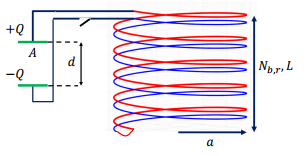
\includegraphics[scale=0.75]{circuit1}
		\end{center}

\noindent In order to solve this problem, we will construct a similar circuit consisting of the capacitor and a single inductor whose inductance is the effective inductance due to the combination of the red and blue components in the picture above. In order to define this effective inductance, first consider an Amperian loop in the z-x plane. We have that: 
	\begin{align*}
		\oint \mathbf{B} \cdot d\vec{l} &= \mu_0 I_{\text{enc}} \\ 
		B l &= \mu_0(n_rI - n_bI)l \\ 
		\mathbf{B} &= \mu_0(n_rI-n_bI) \hat{z} 
	\end{align*}
Now we have the magnetic field inside the inductor. Now let's calculate the magnetic flux through the cylinder given it has a radius of a. We have that: 
	\begin{align*}
		\Phi 	&= \Phi_r + \Phi_b\\ 
				&= \int \mathbf{B} \cdot d\vec{a}  \\ 
				&= B\ell n_r\pi a^2 - B \ell n_b\pi a^2 \\ 
				&= B\pi a^2 \ell(n_r-n_b) \\ 
				&= \mu_0(n_rI-n_bI) \cdot \pi a^2\ell(n_r-n_b) \\ 
				&= I \mu_0 \ell \pi a^2 (n_r - n_b)^2 
	\end{align*}
From this equation we can identify the inductance as: 
	\begin{eqnarray}
		L_{\text{eff}} = \mu_0 \ell \pi a^2 (n_r - n_b)^2
	\end{eqnarray}
Now we can analyze the flow of charge through the equivalent LC circuit shown below: 
	\begin{center}
		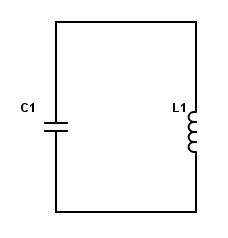
\includegraphics[scale=0.5]{circuit2}
	\end{center}

\noindent From Kirchoff's loop law, we can write the differential equation for the charge in the circuit as follows: 
	\begin{align*}
		L\ddot{Q} + \frac{1}{C}Q &= 0 \\
		\ddot{Q} + \frac{1}{LC}Q &= 0 \\ 
		\text{guess:} \quad Q(t) &= e^{\lambda t}  \\ 
		\Rightarrow \lambda^2 +\frac{1}{LC} &= 0 \\ 
		\lambda = \pm &i\frac{1}{\sqrt{LC}} \\ 
		\text{define:} \quad \omega &\equiv \frac{1}{\sqrt{LC}} \\ 
		Q(t) = c_1 \cos(\omega t) &+ c_2 \sin(\omega t)
	\end{align*}
We are given that $Q(0) = Q_0$ and because the switch is initially open, we have that $\dot{Q}(0)=I(0)=0$. Thus we can say that: 
	\begin{equation*}
		Q(t) = Q_0 \cos(\omega t)
	\end{equation*}
For completeness, I will now substitute in our definition for L into the final equation. Going forward I will continue to use $\omega$ wherever possible for simplicity. Recall that the capacitance for a parallel plate capacitor is given by $C=\frac{\epsilon_0 A}{d}$. Therefore: 	
	\begin{align*}
		\omega 	&= \frac{1}{\sqrt{LC}} \\ 
				&= \frac{1}{\sqrt{(\frac{\epsilon_0 A}{d})(\mu_0 \ell \pi a^2 (n_r - n_b))}}	 \\ 
		\Rightarrow Q(t) &= Q_0 \cos\Bigg(\frac{t}{\sqrt{(\frac{\epsilon_0 A}{d})(\mu_0 \ell \pi a^2 (n_r - n_b)^2)}}\Bigg)
	\end{align*}
For later reference taking one time derivative gives the current: 
	\begin{equation*}
		I(t) = -\dot{Q}(t) = \omega Q_0 \sin(\omega t) = I_0sin(\omega t)
	\end{equation*}

Now to calculate the energy stored in the inductor and capacitor we have the following equations: 
	\begin{align*}
		U_L &= \frac{1}{2}LI^2 \\ 
			&= \frac{1}{2}L\omega^2 Q_0^2\sin^2(\omega t) \\ 
		U_C &= \frac{1}{2}\frac{Q^2}{C} \\ 
			&= \frac{1}{2}\frac{1}{C}Q_0^2cos^2(\omega t)
	\end{align*}
Now for the total energy, recall that $L\omega^2 = \frac{1}{C}$. Thus we have that: 
	\begin{align*}
		U_T &= U_L + U_C \\ 	
			&= \frac{1}{2}L\dot{Q}^2 + \frac{1}{2}\frac{1}{C}Q^2 \\ 
			&= \frac{1}{2}\frac{Q_0^2}{C}\sin^2(\omega t) + \frac{1}{2}{Q_0^2}{C}\cos(\omega t) \\ 
			&= \frac{1}{2}\frac{Q_0^2}{C}
	\end{align*}
Which we can see does not vary in time. \\ 

\noindent Now for part (3) we know that current was not flowing before the switch was closed. This means that after the switch is closed, charge wants to move from the +Q end to the -Q end and so therefore current is not constant forever. This implies that both the electric and magnetic fields will be functions of time and therefor we must consider Faraday's law and Ampere's law (with Maxwell's correction): 
	\begin{align*}
		\nabla \times \mathbf{E} &= -\partial_t \mathbf{B} \\ 
		\nabla \times \mathbf{B} &- \mu_0\epsilon_0\partial_t\mathbf{E} = \mu_0 \vec{J} 
	\end{align*}
The Poynting vector is defined as: 	
	\begin{align*}
		\vec{S} \equiv \frac{1}{\mu_0}(\mathbf{E} \times \mathbf{B})
	\end{align*}
From class (and in Griffiths) we know that: 
	\begin{equation*}
		\partial_t(u_{\text{mech}}+u_{\text{EM}}) = -\nabla \cdot \vec{S}
	\end{equation*}
Which essentially states that any change in time of the mechanical and EM energy densities can be attributed to the flux of the Poynting vector leaving the volume. We can calculate 
the divergence of the Poynting vector as follows: 
	\begin{align*}
		-\nabla \cdot \vec{S} &= -\nabla \cdot (\frac{1}{\mu_0}(\mathbf{E} \times\mathbf{B})) \\ 
				&= -\frac{1}{\mu_0}\Big[(\nabla \times \mathbf{E})\cdot \mathbf{B} - (\nabla \times \mathbf{B})\cdot \mathbf{E}\Big] \\ 
				&= -\frac{1}{\mu_0}\Big[-\partial_t\mathbf{B}\cdot \mathbf{B} - \epsilon_0\mu_0\partial_t\mathbf{E}\cdot\mathbf{E}\Big]  \\ 	
				&= \frac{1}{\mu_0}\Big[\partial_t\mathbf{B}\cdot \mathbf{B} + \epsilon_0\mu_0\partial_t\mathbf{E}\cdot\mathbf{E}\Big]\\
		\Rightarrow -\nabla \cdot \vec{S} &> 0 				
	\end{align*}

\section*{Trajectory} 
Recall from problem 1 that we have shown  $Q(t) = Q_0\cos(\omega t)$. Now in between the plates of the capacitor we have that there is no current moving-- it's just vacuum. So Maxwell's equation for Ampere's law becomes: 
	\begin{equation*}
		\nabla \times \mathbf{B} = \mu_0\epsilon_0\partial_t \mathbf{E} 
	\end{equation*}
Now, to find the electric field in the capacitor, we will use a Gaussian pillbox around the top plate. Thus: 
	\begin{align*}
		\int \mathbf{E} \cdot d\vec{a} &= \frac{1}{\epsilon_0}Q_{\text{enc}} \\ 
		EA &= \frac{1}{\epsilon}Q \\ 
		\Rightarrow \mathbf{E}(t)&= \frac{1}{\epsilon_0 A}Q(t)(-\hat{z})\\ 
		&= -\frac{Q_0\cos(\omega t)}{\epsilon_0 A}\hat{z}
	\end{align*}	
Now that we have \textbf{E} we can find \textbf{B} using an Amperian loop of radius r. 
	\begin{align*}
		\int (\nabla \cdot \mathbf{B})\cdot d\vec{a} &= \mu_0\epsilon_0\int\partial_t \mathbf{E} \cdot d\vec{a} \\ 
		\int \mathbf{B}\cdot d\vec{l} &= -\mu_0\epsilon_0\partial_t E \pi r^2 \\
		B2\pi r &= -\mu_0\epsilon_0\partial_t E \pi r^2  \\ 
		B &= =\mu_0\epsilon_0\frac{\dot{Q}r}{2\epsilon_0 A} \\ 
		\mathbf{B} &= \frac{-\mu_0 \dot{Q}(t)r}{2A}\hat{\phi} \\
					&=\frac{-\mu_0 \dot{Q}(t)\sqrt{x^2+y^2}}{2A}(-sin(\theta)\hat{x} + \cos(\theta)\hat{y}) \\ 
					&= \frac{\mu_0\omega Q_0 \sin(\omega t)\sqrt{x^2+y^2}}{2A}(-\sin(\theta)\hat{x} + \cos(\theta)\hat{y})
	\end{align*}
The last line uses $\theta = \arctan(y/x)$ to define an angle in the plane. Now we can define the force on the electron as: 
	\begin{equation}
		\mathbf{F} = -e\big[\mathbf{E}(t) + \vec{v}\times\mathbf{B}(t)\big]
	\end{equation}

\noindent There is one special case to think about for this equation... the low hanging fruit if you will. That is when x=y=0. This forces the magnetic field to be zero and consequently, the motion is only along the z axis as determined by \textbf{E}. For any case more interesting, numerical methods are almost necessary as solving the second order ODE (Newton's second law) is extremely difficult. Attached is python code for solving for the trajectory using Euler's method twice (ran out of time before I could try Verlet's method). For a initial velocity of zero and an initial position of $\vec{r} = 0.25\hat{x} + 0.25\hat{y} + 0.0\hat{z}$ the following trajectory was produced: 
	\begin{center}
		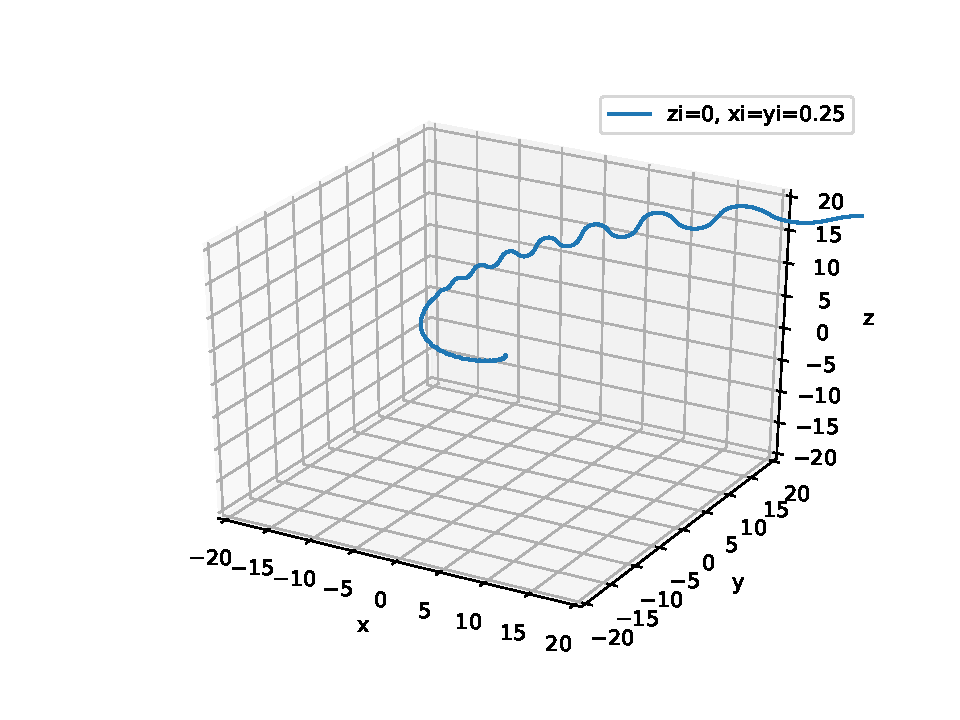
\includegraphics[scale=1.0]{trajectory}
	\end{center}
Note that we are considering an electron which has negative charge. Thus there is a distinct 'towards the top' bias. The oscillations in the z direction begin small and increase, likely because once v becomes significantly large there is a non-zero component of the magnetic force (due to the cross product of $\vec{v}, \mathbf{B}$) that interacts with the electric force. 



























































\end{document}































